\ESKDappendix{����������}{������ US3615068A\label{app:D}}

\begin{figure}[ht!]
	\centering
	
\includegraphics[width = 0.5\textwidth]{images/prilD} 
	\label{prilD}
\end{figure}

A PRECISION ROTARY TABLE FOR USE IN ELECTRO-OPTICAL RE-SEARCH INCLUDES A STATIONARY BASE MEMBER AND A MOVABLE SUPPORT PART OPERATIVELY CONNECTED TO THE BASE MEMBER AND ROTATABLE RELATIVE THERETO. PRECISE POSITIONING OF THE MOVABLE PART IN RESPONSE TO ACTUATION OF A MANUALLY OPERATED MEANS IS EFFECTED BY EMPLOYING GEARING MECHANISM IN WHICH THE VA-RIOUS ROTATING PARTS ARE CONTINUOUSLY SUBJECTED TO A CONSTANT FORCE IN A DIRECTION SUCH THAT THE MESHING GEARS ARE PLACED IN BACK-LASH-FREE ENGAGEMENT WITH EACH OTHER. AN ATTACHMENT DEVICE MAY BE ROTATABLY CONNECTED TO THE MOVABLE PART, THAT DEVICE INCLUDING MECHANISM WHICH PERMITS QUICK MOVEMENT OF THE ATTACHMENT DEVICE BETWEEN TWO PRESELECTED POSITIONS.\par

\newpage

\begin{figure}[ht!]
	\centering
	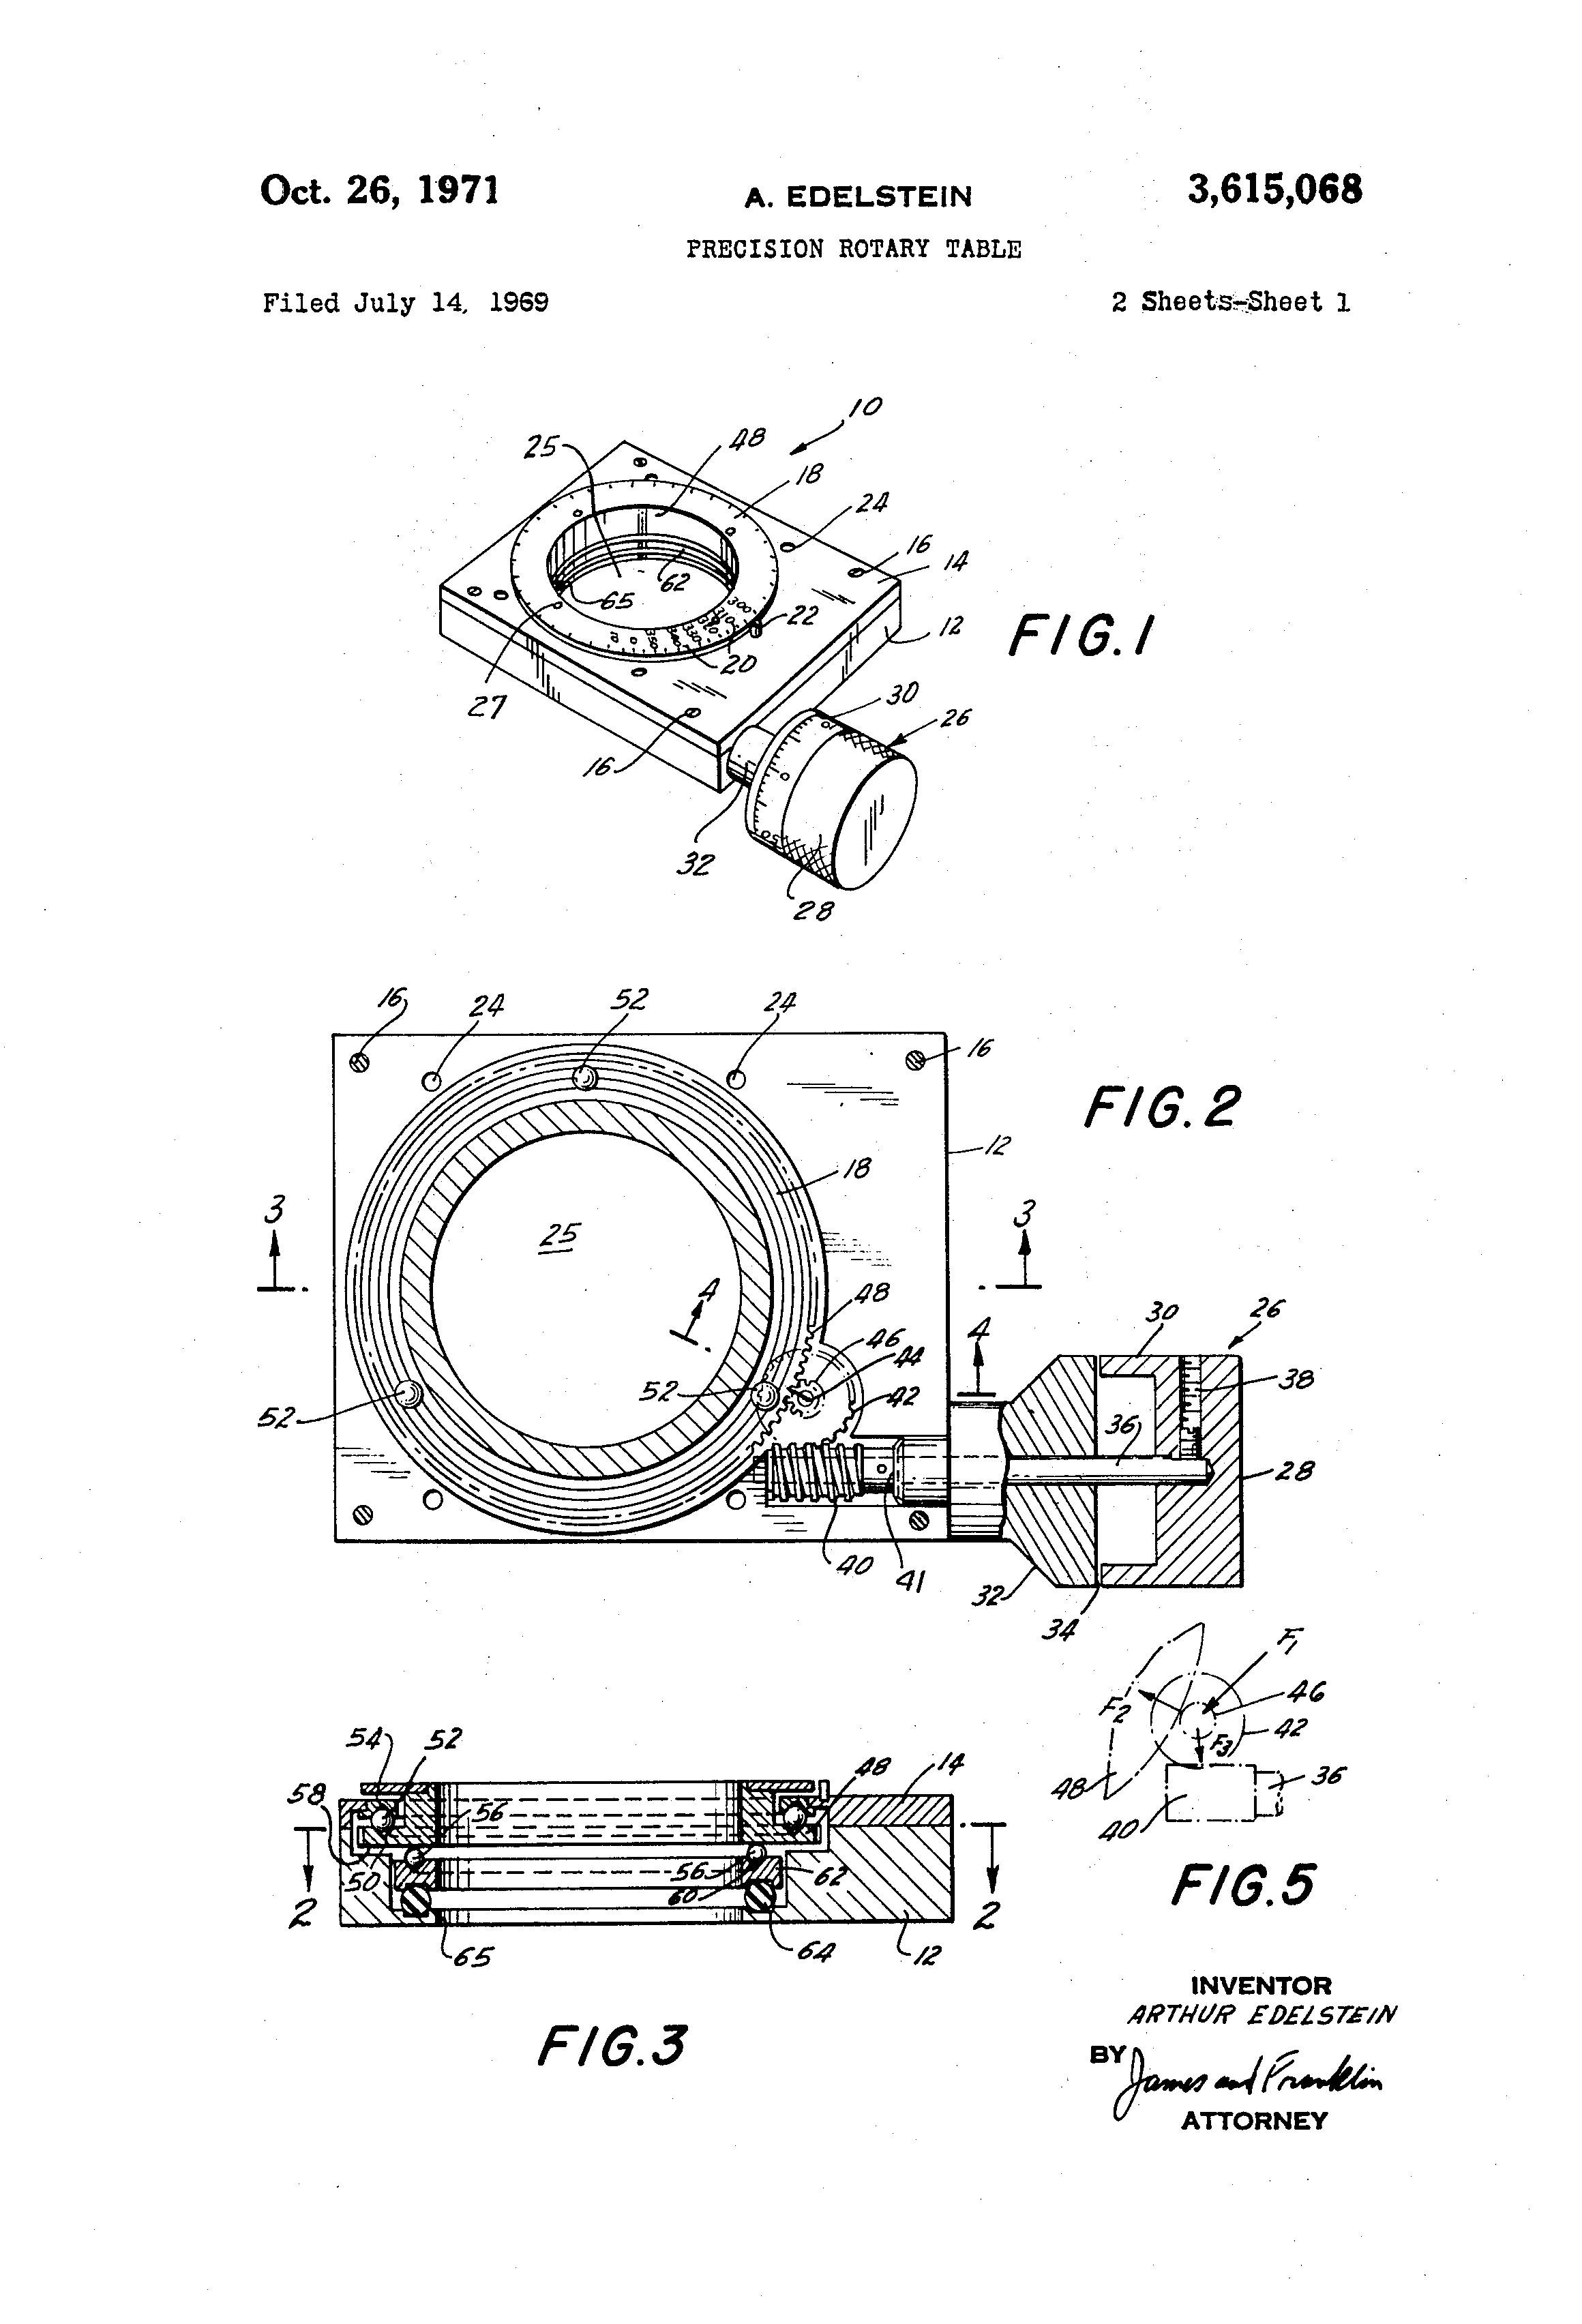
\includegraphics[width = 0.9\textwidth]{images/prilD_1} 
	\label{prilD_1}
\end{figure}
